\chapter{Research Methodology}
\label{cha:research-methodology}

The aim of this chapter is to present the research methodology adopted during the work described in this thesis. Not all the methods have been explicitly elaborated in the papers included in Part II, but they have been nevertheless important while framing the studies and designing the tools employed during my research.


\section{Research Philosophy}

The leading research philosophy adopted was \textit{phenomenology}, a variation of \textit{interpretivism}. According to the interpretivist approach, it is important for the researcher as a social actor to appreciate differences between people \autocite{saunders_research_2009}. Studies adopting the interpretivism research philosophy usually focus on meaning and may employ multiple methods in order to reflect different aspects of the issue. During my research, quantitative data were collected and used to validate theories and outcomes; however, we could not refrain from considering subjective human interests and meanings to validate the results.

The \textit{phenomenology} branch describes the philosophical approach asserting that what is directly perceived and felt is considered more reliable than explanations or interpretations in communication \autocite{remenyi_doing_1998}. Ideas and theories are generated from a rich amount of data mainly by means of induction, whereas stakeholder perspective may have its reflection on the study.


\section{Design as Research}

The topics proposed in Chapter~\ref{cha:introduction} have been researched using design science research and researching design methods \autocite{hevner_design_2010}.
Design as Research encompasses the idea that performing innovative design that results in clear contributions to the knowledge base constitutes research \autocite{hevner_design_2010}. Knowledge generated via design can take several forms, including constructs, models, methods and instances \autocite{march_design_1995}.
Design as Research thus provides an important strand of research that values research outcomes that focus on the improvement of an artefact in a specific domain as the primary research concern, and then it seeks a broader, more general understanding of theories and phenomena surrounding the artefact as an extended outcome \autocite{hevner_design_2010}.
A key insight into how to perform design science research can be gained by understanding the existence of three design science research cycles in any design research project, summarised in Fig.~\ref{fig:design-cycles} and further detailed by Hevner and Chatterjee \autocite*{hevner_three_2007}.

\begin{figure}[ptb]
    \centering 
	\includegraphics[width=\textwidth]{design}
	\caption{Schema of the three design science research cycles, based on Hevner's model \autocite*{hevner_three_2007}.}
	\label{fig:design-cycles}
\end{figure}


\subsection{Relevance Cycle}
The relevance cycle initiates design science research with an application context that not only provides the requirements for the research (e.g. the opportunity/problem to be addressed) as inputs but also defines the acceptance criteria for the ultimate evaluation of the research results \autocite{hevner_design_2010}.
This process connects design science research with the application context. The iteration allows for improvements and refinements of the requirements and for validating incremental results using field testing feedback.

During my work, a user-centred approach characterised the work pertaining to this cycle. Data collected during user studies contributed to the process of constant refinement and improvement of the tools and technologies designed.

\subsection{Rigor Cycle}
The rigor cycle ensures that research is grounded in relevant literature and has solid foundations. This includes considering the state of the art, past knowledge is in fact essential to drive and support innovative research. A literature mapping on topics relevant to my research was conducted as part of this cycle. This represented the starting point, building a solid knowledge foundation and theoretical background for subsequent research.
Design science research can also contribute to improving the state of the art and the knowledge base. This way, the rigor cycle loop is then closed, providing a tangible contribution to the field of research.

\subsection{Design Cycle}
The internal design cycle is the heart of any design science research project. This cycle of research activities iterates more rapidly among the construction of an artefact, its evaluation and the subsequent feedback to refine the design further \autocite{hevner_design_2010}.
It is important to note the difference between the design cycle and the relevance cycle. The first iterates and validates the artefact against the requirements, whereas during the second the objects of the iteration and refinement are the requirements themselves, not the artefact.
The design cycle should be well balanced between the building and evaluation processes. Scarce commitment in one of the two phases will lead to poor overall results.
The design cycle is quite independent of the relevance and rigor cycles, and it is also executed more.


\section{Research Strategy and Methodological Choice}
\label{sec:research-strategy}

In order to implement the main research strategy, several methods have been adopted. A mix of qualitative and quantitative research methods have been used to account for the unpredictability in field studies \autocite{rogers_why_2007}. Mixed methods research fit well with the research objectives because of its potential with respect to understanding and explaining complex organisational and social phenomena \autocites{cao_interactions_2006}{mingers_combining_2001}.
Further, mixed methods research has received much attention in the social and behavioural sciences recently (for a review, see \cite{tashakkori_mixed_2008}).
During my research inquiry, observations, notes and video and audio recordings were the primary means used to collect data during the field studies with the users (Fig.~\ref{fig:user-study}). Pre-post questionnaires, interviews, quiz games and focus groups were usually employed to evaluate the artefacts employed and the process adopted and to assess the perceived outcome of the user experience.

\begin{figure}[ptb]
    \centering 
	\includegraphics[width=\textwidth]{camera}
	\caption{Video recording of the user interaction occurring around the Tiles cards and cardboard. The brainstorming workshop pictured was one of the studies included in P4.}
	\label{fig:user-study}
\end{figure}

\section{Research Activities}

During the progress of my research, different activities and outcomes contributed to the three cycles of the \enquote{Design as Research} methodology: \emph{relevance}, \emph{design} and \emph{rigor} cycles.

As a first step, I performed a literature mapping of the technological applications in smart cities (P1). The identified needs, challenges and research opportunities were used to drive and support the following steps.
Early design ideas were turned into exploratory low-fidelity prototypes and tested on the field with the users.
Subsequent iterations both improved and specialised the prototypes, building on the experience matured during the field studies and the domain knowledge acquired while mapping the literature.

The central course of my research concentrated on the user evaluation of different prototypes targeting the \textit{idea generation} and \textit{design} phases of the Tiles IoT framework process. Other activities involved the design, creation and evaluation of technological tools connecting and extending the \textit{design} phase into \textit{rapid prototyping}. Fewer iterations were performed on such tools because of the increased complexity of the manufacturing process. However, valuable insights, prototypes, design recommendations and knowledge resulted as an outcome. Working prototypes were also used to validate and extend theories as part of the \emph{rigor cycle}.
Research outcomes were reported in academic publications (Chapter~\ref{cha:results}) and research contributions (Chapter~\ref{cha:contributions}) emerged. Throughout the process, the literature on co-design and tangible interaction (Chapter~\ref{cha:theory}) informed the design work.

\subsection{User Studies}
\label{sec:user-studies}

The primary investigation method selected to understand the domain, familiarise with the target users and evaluate the artefacts produced during the design cycle was \emph{design workshops} (Fig.~\ref{fig:workshop}). These workshops were used both to validate the tools employed and to inform the next design iteration. Insights pertaining to possible improvements or defects were gained from direct experience in the field and extracted from the data collected during the workshops.

\begin{figure}[ptb]
    \centering 
	\includegraphics[width=\textwidth]{workshop}
	\caption{A design workshop with university students, part of the studies included in P3.}
	\label{fig:workshop}
\end{figure}

The typical setting for the majority of the studies was a design workshop where participants worked in groups of two to six people. The objective for most of the workshops was to generate a design idea for an IoT application, adapted to solving a particular problem for a specific end-user. The IoT application idea included the use of smart objects designed by the participants during the workshop. During some of the workshops, the participants continued after this initial idea generation phase, physically building the smart objects embedding sensors and actuators. These smart objects were then programmed by the participants to expose high-level functions to the end-users.

The workshop participants were usually students from secondary school up to university level, aged between 13 and 27. Several workshops were also conducted with other categories of users, including researchers, IT professionals, urban planners, teachers and municipality employees. More than 25 workshops were run between August 2016 and April 2018, with more than 500 participants involved.

Observations, researcher notes and questionnaires were the primary means to collect data. In addition, video recordings, interviews and pictures of the produced artefacts were collected during some of the workshops. My role during the workshops was to present the activities and introduce the concepts of IoT and augmented objects. Later on, during the creative phase, my main task was to observe the work of the group, without intervening. The participants occasionally asked for clarifications or support, in which case I was available to provide the required help.

Data collected was analysed with mixed research methods \autocite{venkatesh_bridging_2013}. The focus of the analysis was twofold. At first, it allowed validating the perceived usefulness, acceptance and learning outcome of the tools used. The outcome of the data analysis also validated the modifications made to the tools, closing the \emph{design cycle}.
The second purpose of the analysis was to spot any usability issue, either in the tools or in the process adopted. Such issues might include confusing guidelines, inappropriate terminology or unclear purpose of the tools at use. These outcomes fed the subsequent iteration of the \emph{design cycle}.

\subsection{Design Iterations}
\label{sec:prototypes}

The work on design and prototyping was driven by the theories adopted and the requirements refined during the user studies. The design process followed a UCD approach \autocites{maguire_methods_2001}{gulliksen_key_2003}. A total of eight prototype iterations were completed. Table~\ref{tab:prototypes} shows an overview of the prototypes created and the technologies used during development in relation to the papers that describe the work.

In order to support the idea generation and prototyping journey, several tools were developed during the Tiles project:

\begin{enumerate}
    \item Several decks of cards, a tabletop cardboard to scaffold the use of the cards and a workshop protocol to guide the process, supporting the problem definition, brainstorming and design phases.
    \item A cloud-based software back-end and development environment to programme the IoT application logic.
    \item Two Bluetooth electronic devices embedding sensors and actuators, supporting rapid prototyping for IoT through object augmentation.
    \item A multi-platform mobile app to facilitate the deployment of the prototypes, serving as a gateway connecting the Bluetooth devices to the cloud software platform.
\end{enumerate}

I contributed to different levels in the design, formalisation of the process, development and scientific evaluation of the components described above, in collaboration with other students and researchers involved in the Tiles project.

\begin{table}
	[!p] \centering \caption{List of prototypes built} \label{tab:prototypes} 
	\begin{threeparttable}
		\begin{tabular}{@{}llllllll@{}} 
			\toprule 
			& & & & \multicolumn{3}{l}{Development}  \\
			\cline{5-7} \noalign{\smallskip} 
			\specialcell[b]{ID\\Ver.} & Name & Released & Prototyping tools & 
			\begin{turn}
				{90}Software
			\end{turn}
			& 
			\begin{turn}
				{90}Hardware
			\end{turn}
			& 
			\begin{turn}
				{90}Material
			\end{turn}
			& Papers \\
			\midrule \noalign{\smallskip} 
			D1 & Tiles & Aug-16 & Personas, Scenarios & & & \textbullet & P2 \\
			D2 & Tiles SC & Jan-17 & Cards, Cardboard & & & \textbullet & P3, P5 \\
			D3 & Tiles Ref & May-17 & Storyboard, Personas & & & \textbullet & P4 \\
			\hline \noalign{\smallskip} 
			W1 & RapIoT App & Jun-17 & Android/iOS framework & \textbullet & & & P6 \\
			W2 & Tiles Temp v1 & Feb-18 & Arduino, Electronics & \textbullet & \textbullet & & Internal \\
			W3 & Tiles Temp v2 & Mar-18 & Electronics & & \textbullet & & P7 \\
			W4 & RapIoT Cloud & Apr-18 & Javascript Node.js & \textbullet & & & P7 \\
			W5 & Tiles Square & Apr-18 & Arduino Firmware & \textbullet & & & P7 \\
			\bottomrule 
		\end{tabular}
		\begin{tablenotes}
			\item
			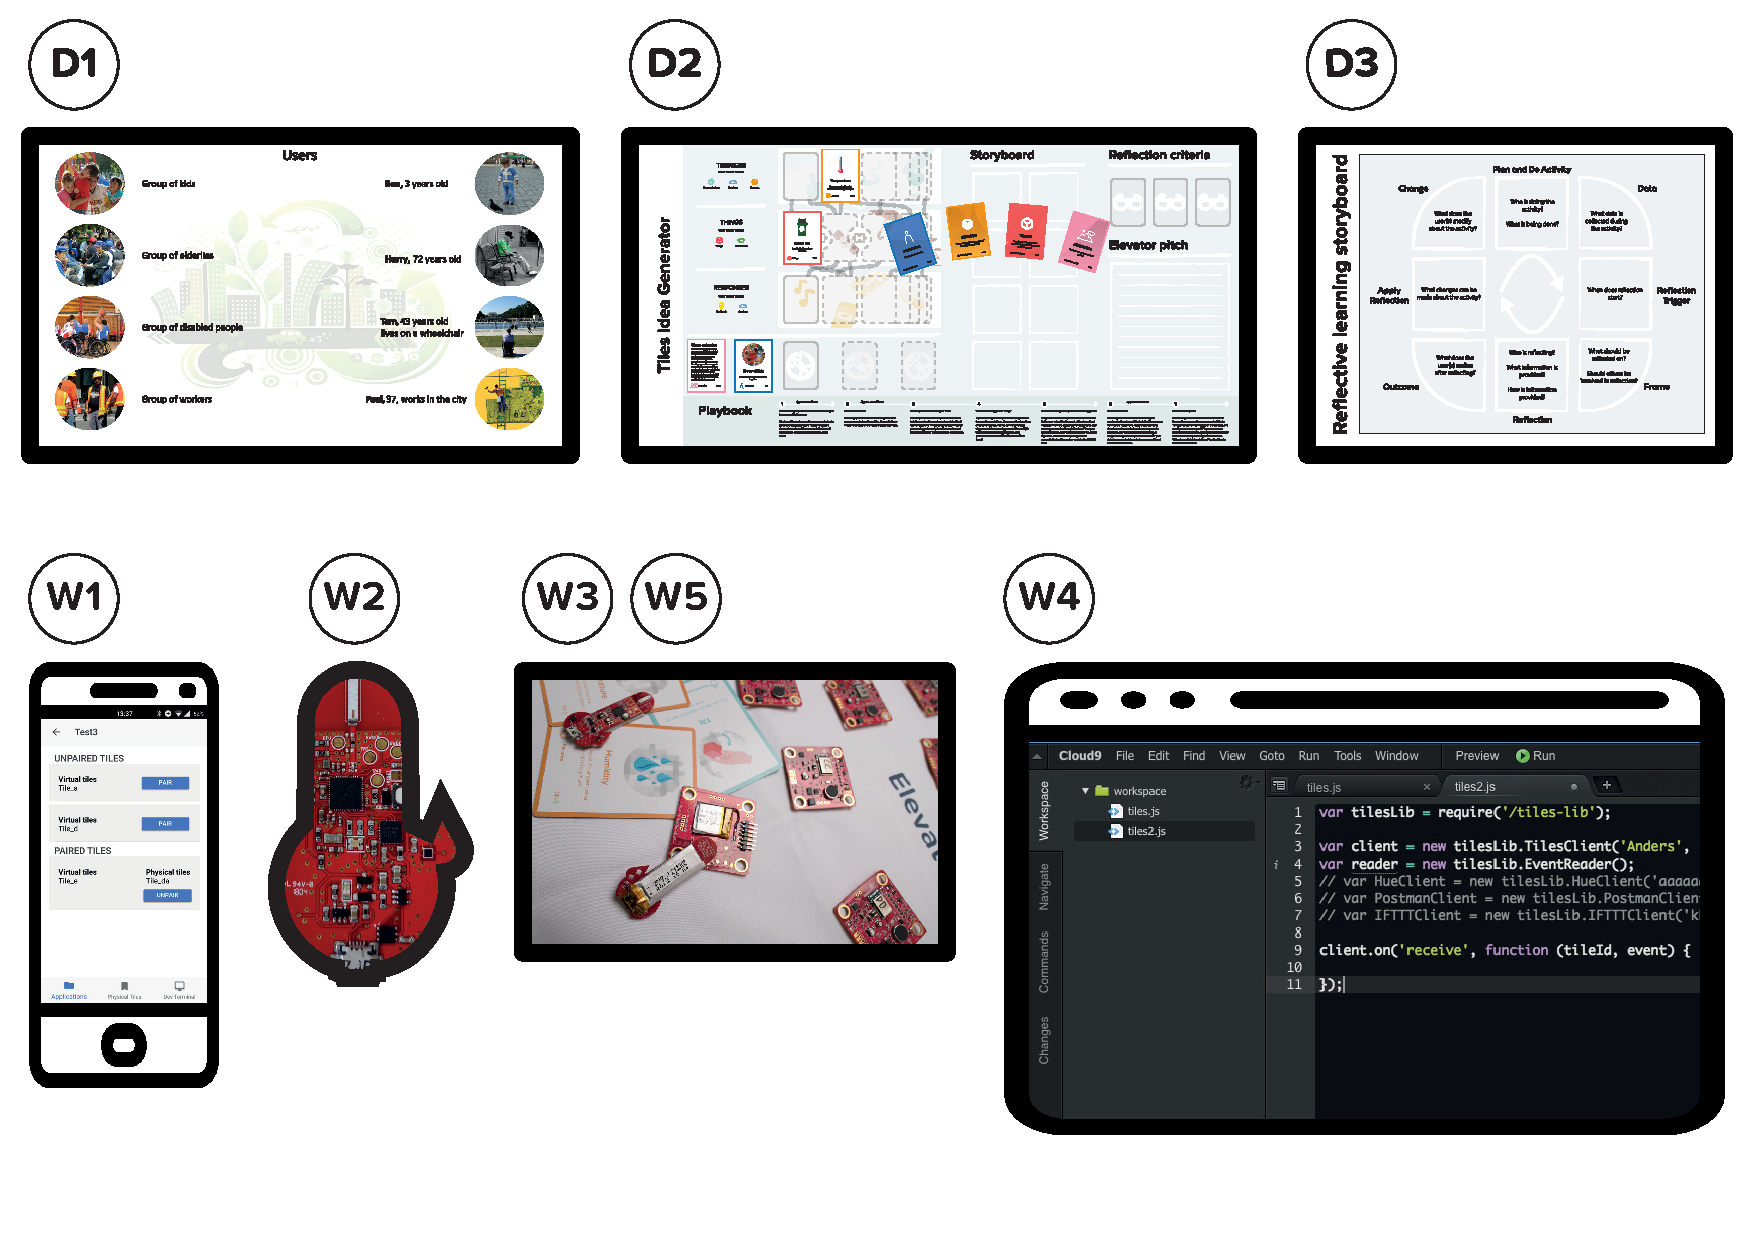
\includegraphics[width=\linewidth]{proto}
		\end{tablenotes}
	\end{threeparttable}
\end{table}

Building the prototypes involved a mix of design, software, hardware and material development. Software was written to create the cloud-based development environment and back-end, the mobile application, and to programme the microcontroller embedded in the electronic devices. The hardware development included the design, manufacturing and testing of electronic boards with embedded sensors and actuators (Fig.~\ref{fig:pcb}). The cards and the tabletop board were designed using desktop publishing and vector graphic editor software. The cards were printed on standard paper, on cardboard and finally on professional-grade playing-card material. The tabletop board was printed on paper, cardboard and various textile materials.

\begin{figure}[ptb]
    \centering 
	\includegraphics[width=0.7\textwidth]{pcb}
	\caption{Details of the CAD circuit board of the Tiles Temp v2. The temperature and humidity sensors are located in the two dashed areas.}
	\label{fig:pcb}
\end{figure}

Design iterations were usually quick. As soon as incremental improvements and feedback were gathered, a new prototype was produced and tested on the field. Some of the software tools employed included Arduino\footnote{https://arduino.cc} for microcontroller development, the Adobe Creative Cloud suite to design the cards and the cardboard and the Ionic framework to create the mobile application.
Traditional and rapid prototyping approaches complemented the work. The electronics were designed in-house using the Eagle CAD software and built by an external electronics manufacturing company. An external company also printed the cards and the tabletop board in their final version.

After each iteration on the prototypes, an evaluation during a workshop was performed. User testing allowed for maintaining a user-centred design perspective, to introduce new ideas into the process, fix defects and validate the new changes. Some prototypes were built only for internal testing purposes (W2). The Tiles cards, cardboard and workshop process were also part of an expert evaluation in October 2018, where 15 professional designers and IoT researchers from all around Europe provided feedback and suggestions after experimenting with the toolkit during a brainstorming workshop.


\section{Research Approach in Field Studies}

The research approach employed during the investigation described in this thesis is here evaluated and contextualised. A research strategy based on case studies was adopted. Case studies focus on understanding the dynamics present within single settings \autocites{eisenhardt_building_1989}. During my research, this research strategy was supported by a methodology based on mixed methods, as motivated in Section~\ref{sec:research-methodology}. Validity and reliability issues within case studies \autocites{yin_case_2017}{riege_validity_2003} are also discussed.

Criteria were established for judging the quality of the case study strategy \autocite{riege_validity_2003}. Several tests and techniques were synthesised for establishing validity and reliability in case study research, as well as the validity of the mixed methods methodology.
In the following section, the research approach is evaluated following the guidelines and design tests reported by Riege \autocite*{riege_validity_2003}; however, not all the tests devised by Riege apply to the studies in the articles included in this thesis.

\subsection{Construct Validity}
Construct validity evaluates whether appropriate operational measures have been adopted for the theoretical concepts being researched.
Collecting data using multiple data sources increases construct validity and protects against researcher bias \autocites{perakyla_reliability_1998}{flick_triangulation_1992}. Converging findings emerged when analysing different sources through triangulation. This has been the case for the data collected during the evaluation workshops reported in all the articles except P1, where there was no workshop-based empirical evaluation. We collected quantitative and qualitative data through questionnaires, structured interviews, observations, video and audio recordings and analysis of the artefacts produced. Chains of evidence in the data \autocites{griggs_analysing_1987}{hirschman_humanistic_1986} were highlighted when summarising the outcome of the data analysis process. For example, in line with the iterative nature of design as research, evidence collected during the first design iteration in P2 was used to ground and improve tools and processes employed in P3, P4 and P5.

The total number of participants involved in the studies added up to more than 500. A fraction of them were involved in the studies presented in this thesis. Significant experience was gathered in the process, such experience contributed to the definition of theories and in providing insights while analysing qualitative and quantitative data.
The size of the data sample allowed for some statistical analysis, but I looked for confirmation in the qualitative data before formalising the results. Given the number of human factors involved, this strategy was demonstrated to be more robust and allowed for better interpretation of the data collected. As an example, some of the dynamics of the study reported in P3 were not observable from a qualitative point of view, while an aggregated quantitative analysis didn't match with the evidence collected through observations. A more in depth analysis on the quantitative data was needed to formulate a plausible explanation of these dynamics.

During the studies, researchers had close and direct personal contact with the organisations and users involved. Effort was then made to refrain from subjective judgements during the periods of research design and data collection, to enhance construct validity. For this reason, results were discussed among the entire research group before formalising theories and constructs. Researchers not directly involved in specific studies were included in the discussion, to provide additional perspective.

Each of the studies was limited to one or two sessions, lasting usually two to three hours each. It was, therefore, not possible to prove long-term effects for the tools developed.

\subsection{Internal Validity}
Internal validity, as traditionally known in quantitative research, refers to the establishment of cause-and-effect relationships, while the emphasis on constructing an internally valid research process in case study research lies in establishing phenomena in a credible way \autocite{riege_validity_2003}. Researchers should not only highlight major patterns of similarities and differences between the experience of the respondents and their beliefs but also try to identify what components are significant for those examined patterns and what mechanisms produced them. An example of the need to assess the significance of these patterns is provided by the data collected during the studies of P2 and P3. In both cases we recorded discording opinions about the desired level of constraints of the design tools employed. Some of the users desired more freedom during the brainstorming session, while others felt overwhelmed by the number of choices. However, during the studies of P2 the pattern was significantly tending towards the need to have more constraints and guidance, while during the studies of P3 the pattern was not significantly pointing to any of the two cases.

Data from the field studies included in the papers presented in this thesis were checked cross-case to assess the internal coherence of findings \autocite{miles_qualitative_1994}. Illustrations and diagrams eased this task, allowing the identification and evaluation of evidence, cross-checking within-case and cross-case \autocite{yin_case_2017}.

During field studies, it was sometimes required to deviate from the agreed protocol because of unpredictable events. In addition, it was difficult to replicate the same exact conditions because of the human factors involved and the lack of control over some of the variables. Workshops in the classroom were often limited in time, involved a variable number of students and took place at different times of the day.

Despite the challenges, I was able to gather enough evidence to complete the design work. The experience matured was helpful in extracting valuable know-how from noisy data sets.

\subsection{External Validity}
External validity is concerned with the extrapolation of particular research findings beyond the immediate form of inquiry to the general.

While quantitative research, for example, using surveys aims at statistical generalisation and synthesis as methods to pursue external validity, case studies rely on analytic generalisation, whereby particular findings are generalised to some broader theory. The focus lies on an understanding and exploration of constructs, that is, usually the comparison of initially identified and/or developed theoretical constructs and the empirical results of single or multiple case studies \autocite{riege_validity_2003}.

In order to increase the external validity, several techniques were employed. The logic of the case study was replicated across different domains \autocites{eisenhardt_building_1989}{parkhe_messy_1993}: most of the workshops involved students, but the tools were evaluated also with other target users (e.g. in P4), including researchers, employees from the municipality, entrepreneurs, programmers and freelancers. The domain of the study included in P4 is also unique since it was the only study to target IoT application for reflective learning.

The boundaries and scope of the research were defined in the research design phase \autocite{marshall_designing_2014}. The outcome for each of the phases covered by the toolkits was clearly defined, as well as the target users of the toolkits and their attributes (see Chapter~\ref{cha:iot-framework} for details).

Lastly, comparison of evidence with the extant literature in the domain of interest helped in clearly outlining the contributions and in generalising, always within the scope and boundaries of the research \autocite{yin_case_2017}.

\subsection{Reliability}
Reliability refers to the demonstration that the operations and procedures of the research inquiry can be repeated by other researchers who then achieve similar findings; that is, the extent of findings can be replicated assuming that, for example, the interviewing techniques and procedures remain consistent \autocite{riege_validity_2003}.

In case study research, this can raise problems as people are not as static as measurements used in quantitative research, and even if researchers were concerned about ensuring that others can precisely follow each step, the results may still differ. Indeed, data on real-life events, which were collected by different researchers, may not converge into one consistent picture. However, possible differences also can provide a valuable additional source of information about the cases investigated \autocite{riege_validity_2003}.

The techniques used to increase reliability included the recording of observations and actions as concretely as possible \autocite{lecompte_problems_1982}, the use of pilot studies to develop and refine the case study protocol \autocites{eisenhardt_building_1989}{mitchell_industrial_1993}{yin_case_2017}, the use of multiple researchers who continually communicate about methodological decisions \autocite{lecompte_problems_1982}, the mechanical recording of data \autocite{nair_using_1995}, the development of a case study database to organise and document the mass of collected data \autocite{lincoln_naturalistic_1985} and finally the use of peer review and examination \autocite{lecompte_problems_1982}.
These techniques were applied for example by conducting pilot studies prior to the studies included in P2 and P4, by refining the methods in a collaborative manner within our research group, by systematically recording data through pictures of the artefacts and questionnaires, by redacting a spreadsheet containing all the details of each study, including version and type of the tools tested, details about the participants, type of data collected and research objectives.

Repeatability can be demonstrated by the existence of external publications employing the Tiles ideation toolkit in contexts similar to the ones presented in the papers included in this thesis (see Section~\ref{sec:exploitation} for details). In some cases, the ideation process directing the use of the Tiles cards was modified or extended (e.g. removing the cardboard). The results reported, however, are aligned with the findings presented in this thesis.

Relative to repeatability, limitations might affect the prototyping phase. This phase, in fact, was evaluated and tested only internally during the last months of my PhD. External adoption and independent evaluations of the prototyping toolkit are not yet possible because of the early stage of development of the hardware and software stacks.


\section{Ethical Considerations}

Data captured was handled in observance of the Norwegian University of Science and Technology (NTNU) policies. Occasionally younger users received a gift card after participating. In some workshops, the prize was awarded only to the best ideas generated, voted by the participants themselves. All the users involved in the studies signed a consent form which explained how the collected data was used. Younger users were required to have the consent form signed by a parent or a tutor. All the data collected was anonymised, kept confidential and not disclosed to third parties. Data contained in the articles thus do not include any information that can lead to the identification of a specific data subject. All the users were given the opportunity to withdraw their consent at any time and the data was destroyed after being analysed.
While deciding which type of data to collect, we followed a \textit{privacy by design} approach \autocite{cavoukian_privacy_2009}, considering the data collected as a liability and not as an asset. In addition, compliance of data collection and handling with national legislation was assured by enforcing the regulations mandated by the Norwegian Centre for Research Data (NSD\footnote{https://nsd.no/}).


\section{User Centred Design Approach}

In order to create more meaningful solutions, which are better tailored to the wishes and needs of the final users, designers have become more concerned about the stakeholders of their creations \autocite{sanders_co-creation_2008}. In the landscape of human-centred design, UCD is one of the approaches that can help in that direction.
UCD and co-design involve value creation in ongoing, productive collaboration with all relevant parties, with end-users playing a central role \autocite{jansen_7_2017}.

Benyon \autocite*{benyon_designing_2014} distinguished four ways in which UCD pays off:
\begin{itemize}
    \item With close user involvement, products are more likely to meet the expectations of the users and their requirements. This leads to increased sales and lower costs incurred by customer services.
    \item System designers tailor products for people in specific contexts and with specific tasks, thereby reducing the chances of situations with a high risk of human error arising. UCD leads to safer products.
    \item Putting designers in close contact with users means a deeper sense of empathy emerges. This is essential in creating ethical designs that respect privacy and quality of life.
    \item By focusing on all users of a product, designers can recognise the diversity of cultures and human values through UCD, a step in the right direction towards creating sustainable businesses.
\end{itemize}

UCD is a design approach that foresees the active involvement of the stakeholders during the design process. Users play the role of \textit{experts of their experience} and participate in knowledge and idea development \autocite{sanders_co-creation_2008}. Research suggests that more innovative solutions can be obtained when co-design techniques are adopted \autocite{trischler_value_2018}, while end-users are believed to have a better perspective of the problem at stake compared to designers, who are not necessarily familiar with the domain addressed as they are with the design methods used to tackle the problem.

Lockton et al. \autocite*{lockton_designing_2014}, advocated the importance of understanding people. Their contexts and social practices of living and working are seen as fundamental to frame problems appropriately, namely, in a way that corresponds to the real lives of the people, instead of basing it on assumptions.
UCD is an iterative process that aims to understand users and their contexts in all stages of design and development. UCD is pertinent to my work especially in connection to the toolkits produced during my PhD and described in Chapter~\ref{cha:iot-framework}. Multiple iterations were performed on the prototypes of the toolkits, addressing usability issues, extending the functionalities and improving the design. These iterations followed a UCD approach: field evaluations, direct user feedback and observations during field work informed each iteration on the design of the toolkit.
